
\section{Methodology}
\label{methodology}

Our method (Fig. \ref{fig:blk_diag}, Alg. \ref{alg:online_ckrs}) learns a Koopman operator (Sec. \ref{sec:koop_train}), uses it for control design (Sec. \ref{sec:controller_design}), performs fast linear reachability analysis on the closed-loop lifted Koopman dynamics (Sec. \ref{sec:reachability}), and inflates these reachable sets via CP to obtain probabilistic coverage guarantees (Sec. \ref{sec:conformalize_KRS}).

\subsection{Koopman Operator Training}
\label{sec:koop_train}
To solve Prob. \ref{prob:koopman}, we train a Koopman operator model $(\enc, \dec, \ka, \kb)$ on a dataset $\mathcal{D} \doteq \{(x_{0:T}^{(i)}, u_{0:T-1}^{(i)})\}_{i=1}^N$ of open-loop trajectories from a planner $P$ (details in Sec. \ref{sec:experiments}). We use a composite loss $\mathcal{L} = \sum_{i=1}^N(\lambda_1 \mathcal{L}_1^{(i)} + \lambda_2 \mathcal{L}_2^{(i)})$. The first term, $\mathcal{L}_{\text{1}}^{(i)} = \sum_{j=0}^{T} \big[\|x_{j}^{(i)} - \dec (\enc (x_{j}^{(i)}))\|^2 + \|\enc(x_j^{(i)}) - \enc(\dec(\enc(x_j^{(i)})))\|^2\big]$, enforces autoencoder accuracy via state reconstruction error and a latent consistency loss. The second term, $\mathcal{L}_{\text{2}}^{(i)} = \sum_{j=t+1}^{t+H} \big[\| x_{j}^{(i)} - \dec (\check z_{j}^{(i)})\|^2 + \|\enc (x_{j}^{(i)}) - \check z_j^{(i)}\|^2\big]$, where $\check z_j^{(i)} \doteq \ka \check z_{j-1}^{(i)} + \kb u_{j-1}^{(i)}$ and $\check z_0^{(i)}=\enc(x_0^{(i)})$, is a multi-step (horizon $H$) dynamics loss penalizing prediction errors from the linear model ($\ka$, $\kb$) in both latent and state space.The latent consistency term is crucial for long-horizon prediction accuracy. We initialize $\ka$ as identity and $\kb$ with Xavier uniform, train via learning rate annealing and weight decay, and set ($\enc, \dec$) to have ReLU or GELU activations.
\subsection{Koopman Tracking LQR Design}
\label{sec:controller_design}
To reliably imitate state/control reference trajectories generated by the planner $P$ \textit{in the lifted state space} $\mathcal{Z}$, a tracking controller $\pi$ is required to stabilize against initial condition perturbations $x_0 - x_0^\textrm{ref}$ and to reject disturbances due to model error in the learned lifted dynamics $z_{t+1} = \ka z_t + \kb u_t$. To obtain $\pi$, we use the linearity of the lifted dynamics to design a linear quadratic regulator (LQR) that tracks trajectories in $\mathcal{Z}$. Given a reference state-space trajectory $x_{0:T}^{\text{ref}}$ produced by $P$, we map it to the lifted state space as $z_{0:T}^{\text{ref}} \doteq \{\enc(x_t^{\text{ref}})\}_{t=0}^T$. The corresponding feedforward control trajectory $u_{0:T-1}^{\text{ref}}$ which minimizes the lifted-state imitation error is then computed as:
\begin{equation}
\label{eq:u_ff}
u_{t}^{\text{ref}} = \kb^{\dagger} (z_{t+1}^{\text{ref}} - \ka z_{t}^{\text{ref}}),
\end{equation}
where $\kb^{\dagger}$ is the pseudo-inverse of $\kb$. The error states $\delfz_{t} = z_{t} - \zref_{t}$ and controls $\delfu_{t} = u_{t} - \uref_{t}$ follow linear error dynamics $\delfz_{t+1} = \ka \delfz_{t} + \kb \delfu_{t}$, starting from an initial error $\delfz_0 = \enc(x_0) - \zref_0$, where $x_0 \in \B_{\epsilon}(x_{0}^{\text{ref}})$. 
We solve an LQR problem, finding the feedback controls $\delfu_{0:T-1}$ that minimize the finite-horizon quadratic cost $\delfz_T^\top Q_T \delfz_T + \sum_{t=0}^{T-1} (\delfz_t^\top Q \delfz_t + \delfu_t^\top R \delfu_t)$, subject to the linear dynamics $\delfz_{t+1} = \ka \delfz_t + \kb \delfu_t$, where $Q \succ 0$, $R \succ 0$, and $Q_T \succ 0$. In particular, we solve a backward Riccati recursion to obtain the optimal feedback gains $\lqrmat_{0:T-1}$. This yields the tracking control law in the lifted state space \eqref{eq:u_latent_cl}, which can be applied on the nonlinear system \eqref{eq:open_loop_dynamics} as \eqref{eq:u_real_cl} by measuring and encoding the state $x_t$:%, initialized with $P_T = Q_T$,

\begin{minipage}{0.48\textwidth}
\begin{equation}
\label{eq:u_latent_cl}
u_t = \uref_t - \lqrmat_t (z_t - \zref_t),
\end{equation}
\end{minipage}
\hfill
\begin{minipage}{0.48\textwidth}
\begin{equation}
\label{eq:u_real_cl}
u_t = \uref_t - \lqrmat_t (\enc(x_t) - \zref_t).
\end{equation}
\end{minipage}
\subsection{Reachability Analysis for Closed-Loop Koopman Dynamics}\label{sec:reachability}
\looseness-1
The high computational cost of nonlinear reachability motivates our use of Koopman operators. Standard RSOA computation repeatedly overapproximates nonlinearities at each timestep in both $f$ and $\pi$ (which typically must be nonlinear to stabilize $f$), leading to high conservativeness. A $T$-step RSOA requires $2T$ nonlinear function evaluations, causing reachable sets to become vacuously loose as $T$ increases. To reduce conservativeness, partition-based methods split the input set $\overline{\mathcal{X}}_t$, propagate each partition element, and union the result; however, this incurs computational and memory costs that increases with the cardinality of the partition. In contrast, Koopman-based reachability improves scalability and reduces conservativeness without partitioning overhead by reducing the number of nonlinearities. Mapping to the lifted space $\mathcal{Z}$ creates linear dynamics, eliminating the need to bound nonlinearities during propagation. The linear dynamics also permit a linear tracking controller. Consequently, computing an RSOA $\overline{\mathcal{X}}_t$ for any timestep $t$ requires bounding only a single application of the nonlinear encoder ($\enc$) and decoder ($\dec$), reducing the number of nonlinear bounding operations from $2T$ to just $2$. 
To apply this insight formally for RSOA computation, we define the Tracking Koopman Feedback Loop (TKFL), denoted $\tnfl$, as a CG the describes the closed-loop dynamics for tracking $z_{0:T}^{\text{ref}} \doteq \{\enc(x_t^{\text{ref}})\}_{t=0}^T$ in the lifted state space using the feedback control law \eqref{eq:u_real_cl}.  Specifically, the TKFL $\tnfl : \mathcal{X}_0 \times \mathcal{U}^T \times \mathcal{Z}^{T+1} \rightarrow \hat{\mathcal{X}}^{T+1}$ maps the initial state $x_0 \in \B_{\epsilon}(x_{0}^{\text{ref}})$, the feedforward control trajectory $u_{0:T-1}^{\text{ref}}$ \eqref{eq:u_ff}, and the lifted reference $z_{0:T}^{\text{ref}}$ to the decoded trajectory $\hat{x}_{0:T} \doteq \{\dec(z_{t})\}_{t=0}^T$ representing the predicted closed-loop trajectory \eqref{eq:latent_rollout_tnfl} in the original state space, where the lifted states $z_t$ are updated via the closed-loop lifted dynamics \eqref{eq:latent_closed_loop}: 

\begin{equation}
\label{eq:latent_rollout_tnfl}
    \hspace{-23pt}\hat{x}_{0:T} = \{x_0, \{\dec (\tilde f_z(z_t))\}_{t=0}^{T-1}\},
\end{equation}
\begin{equation}
\label{eq:latent_closed_loop}
    \hspace{-30pt} z_{t+1} = \ka z_t + \kb (u_t^\textrm{ref} - G_t(z_t - z_t^\textrm{ref})) \doteq \tilde f_z(z_t).\hspace{-20pt}
\end{equation}

\begin{figure}[ht]
  \centering
  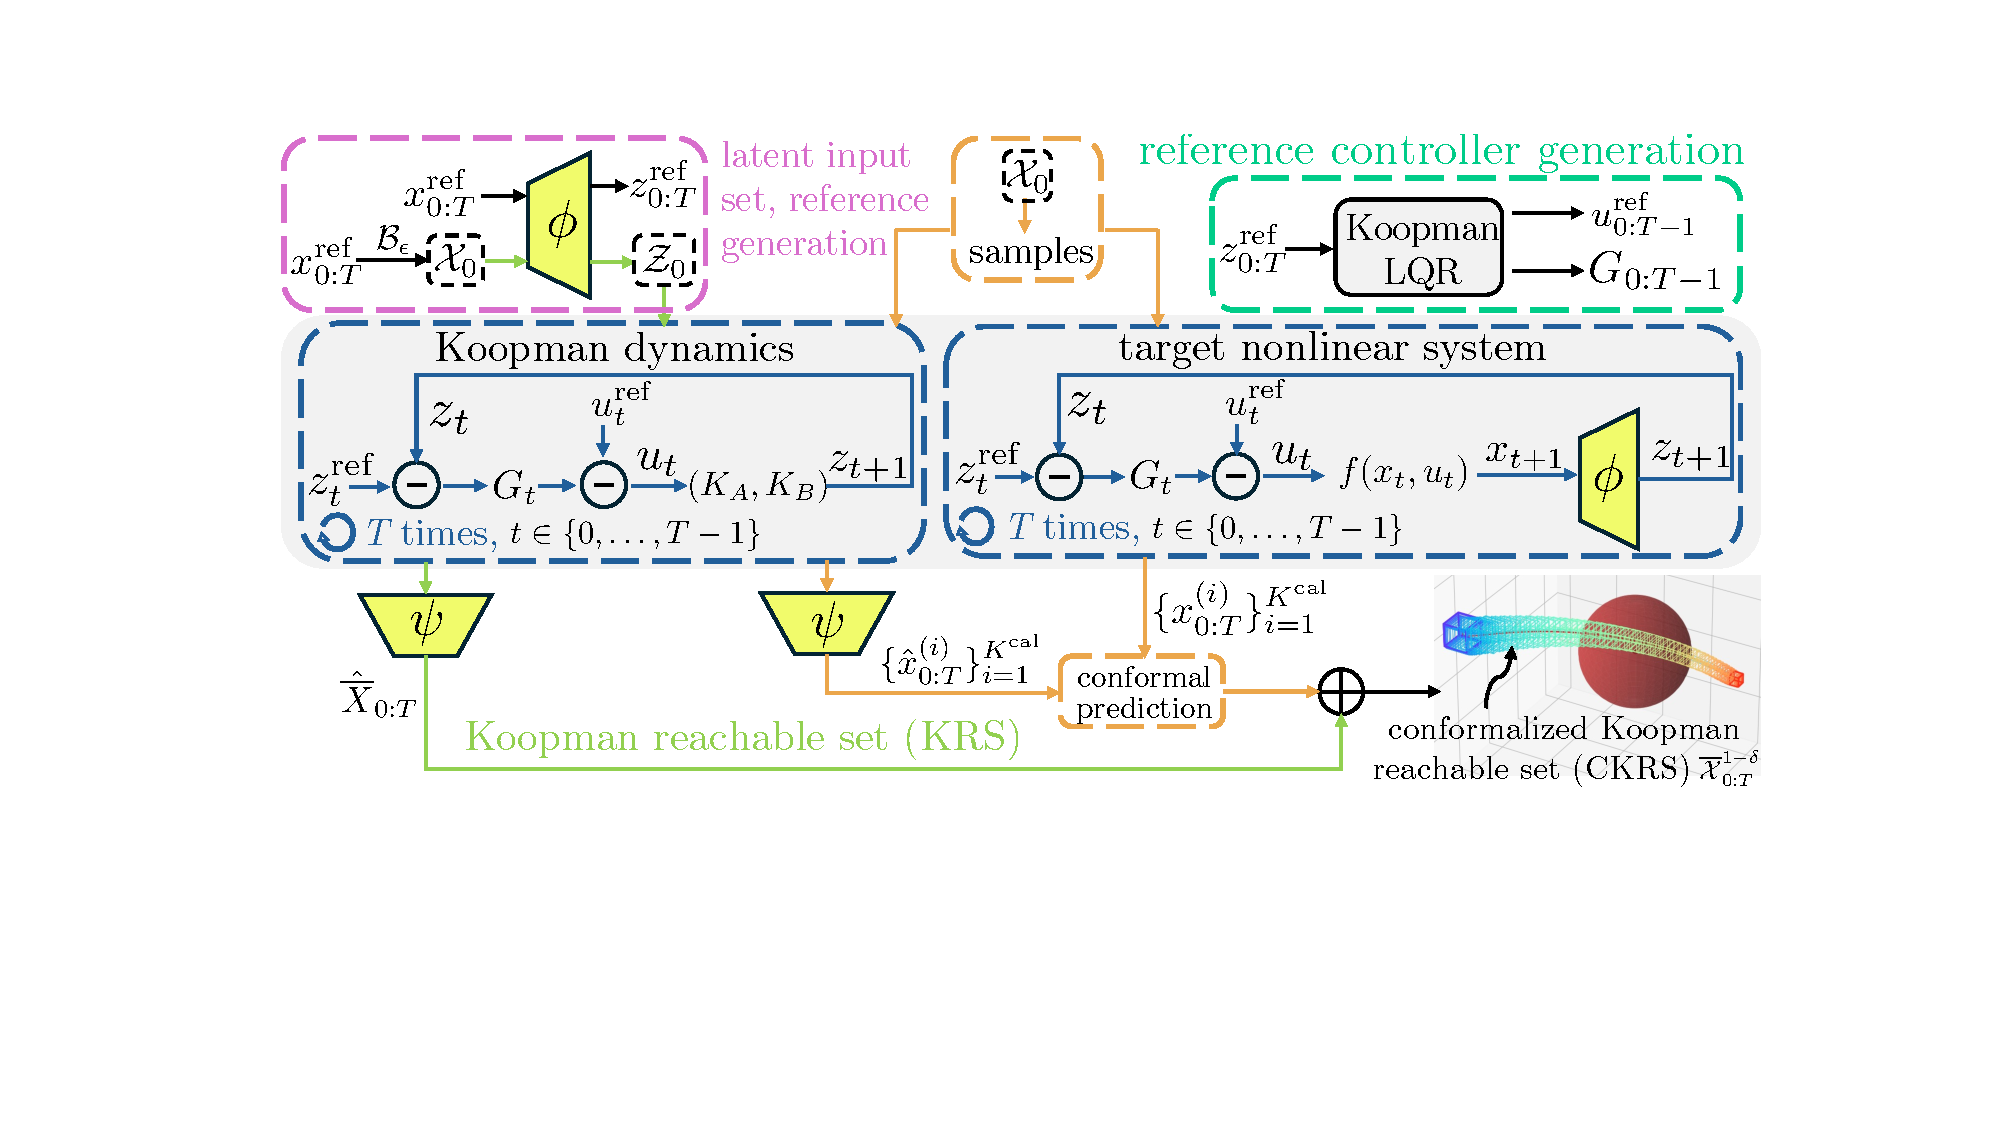
\includegraphics[width=0.85\textwidth]{img/block_diagram_v2.pdf}
  \caption{A block diagram that describes the flow of our method (ScaRe-Kro). Green and orange arrows represent KRS and CP computations, respectively. }
  \label{fig:blk_diag}
\end{figure}

To summarize, the CG is constructed as follows (see Fig. \ref{fig:blk_diag} for visualization). First, we map the initial state via $\enc$ into the latent space, computing $z_0 = \enc(x_0)$. Second, we unroll the $T$-fold recursive application of the single-step latent dynamics, $z_{t+1} = \ka z_t + \kb u_t$,  where $u_t$ is the closed-loop tracking control computed using \eqref{eq:u_latent_cl}, to obtain the latent trajectory $z_{0:T} = \{z_0, z_2, \cdots, z_T\}$. Third, $z_{0:T}$ is mapped back to the original state space via the decoder $\dec$ to obtain $\hat{x}_{0:T}$. 
The CG $\tnfl$ is passed to the \texttt{auto\_LiRPA} library \citep{Xu2020AutoLiRPA}, which enables set-based bound propagation through $\tnfl$ using CROWN \citep{Zhang2018CROWN}. \texttt{auto\_LiRPA} computes vector-valued affine bounding functions, $\underline{\tnfl}$ and $\overline{\tnfl}$, which enables us to compute an RSOA $\hat{\overline{\mathcal{X}}}_{0:T}$ for the decoded closed-loop lifted dynamics \eqref{eq:latent_rollout_tnfl} by considering specific components of $\tnfl$, $\underline{\tnfl}_t$ and $\overline{\tnfl}_t$, that bound the states reached under \eqref{eq:latent_rollout_tnfl} at timestep $t$, starting from any initial condition $x_0 \in {\mathcal{X}}_0$. This resulting hyper-rectangular set $\hat{\overline{\mathcal{X}}}_{0:T}$, which we refer to as the Koopman reachable set (KRS), is found by solving the optimization \eqref{eq:Koopman_RSOA}, which is computed efficiently by \texttt{auto\_LiRPA}:
\begin{equation}\small
    \hspace{-5pt}
    \hat{\overline{\mathcal{X}}}_{0:T} \doteq \big\{ \textsf{Int}\big( \textstyle\min_{\substack{x_0 \in \mathcal{X}_0}} \underline{\tnfl}_t(x_0, \uref_{0:T-1}, \zref_{0:T}), \max_{\substack{x_0 \in \mathcal{X}_0}} \overline{\tnfl}_t(x_0, \uref_{0:T-1}, \zref_{0:T}) \big) \big\}_{t=0}^{T}
    \hspace{-3pt}
    \label{eq:Koopman_RSOA}
\end{equation}
\looseness-1The KRS $\hat{\overline{\mathcal{X}}}_{0:T}$ overapproximates $\hat{x}_{0:T}$ so that $\hat{x}_{t} \in \hat{\overline{\mathcal{X}}}_{t}$, for all $t \in \mathcal{T}$, ensuring the decoded closed-loop lifted dynamics \eqref{eq:latent_rollout_tnfl} remain in $\hat{\overline{\mathcal{X}}}_{0:T}$. Formally, we state the following result (proof in App. \ref{app:proofs}):

\setcounter{theorem}{0}
\begin{lemma}[KRS overapproximation]
\label{lem:koopman_containment}
\renewcommand{\thelemma}{1}
Let $\tnfl$ denote the closed-loop CG of TKFL, and let $\mathcal{X}_0$ be the initial set. Suppose the KRS $\hat{\overline{\mathcal{X}}}_{0:T}$ is defined as in \eqref{eq:Koopman_RSOA}. Then, for any initial state $x_0 \in \mathcal{X}_0$, the decoded closed-loop trajectory \eqref{eq:latent_rollout_tnfl}, i.e.,
$\hat{x}_{0:T} = \tnfl(x_0, \zref_{0:T}, \uref_{0:T-1})$ satisfies $\hat{x}_t \in \hat{\mathcal{X}}_t$ for all $t \in \mathcal{T}$.
\end{lemma}

\looseness-1\noindent Crucially, the KRS overapproximates the reachable set for the decoded Koopman linearized dynamics \eqref{eq:latent_rollout_tnfl}, \textit{not the true nonlinear dynamics} \eqref{eq:closed_loop_dynamics}, due to Koopman model error. This motivates Sec. \ref{sec:conformalize_KRS}.

\subsection{Conformalizing Koopman Reachable Sets}
\label{sec:conformalize_KRS}
\looseness-1
We now explain how to inflate the KRS to guarantee it contains the true system \eqref{eq:closed_loop_dynamics} trajectories with a user-specified probability $1-\delta$. We use CP to compute a high-probability upper bound on the state-space prediction error of the decoded closed-loop lifted dynamics \eqref{eq:latent_rollout_tnfl}. Specifically, we adapt the single nonconformity score approach (SNSA) \citep{cp_survey} to compute state- and dimension-dependent error bounds using a calibration dataset $\mathcal{D}_C = \{(x_{0:T}^{(i)}, \hat x_{0:T}^{(i)})\}_{i=1}^{K^\textrm{cal}}$ of trajectories of the true closed-loop dynamics $x_{0:T}$ \eqref{eq:closed_loop_dynamics} and the decoded closed-loop lifted dynamics $\hat x_{0:T}$  \eqref{eq:latent_rollout_tnfl}. To construct each data tuple in $\mathcal{D}_C$, we sample a reference trajectory $x_{0:T}^{\text{ref},(i)}$ from planner $P$ and an initial state $x_0^{(i)}$ uniformly from $\B_{\epsilon}(x_{0}^{\text{ref}})$. We then compute the latent reference trajectory $z_{0:T}^{\text{ref}, (i)} = \{\enc(x_{t}^{\text{ref},(i)})\}_{t=0}^T$ and the feedforward control sequence $u_{0:T-1}^{\text{ref}, (i)}$ using \eqref{eq:u_ff}. We use $u_{0:T-1}^{\text{ref}, (i)}$ to calculate the trajectory returned by 1) tracking $z_{0:T}^{\text{ref}}$ in the lifted state space (\ref{eq:latent_rollout}) and decoding to the state space via $\dec$ and 2) executing the Koopman controller on the true \textit{nonlinear dynamics} (\ref{eq:actual_rollout}):


\noindent\begin{minipage}[b]{0.54\textwidth}
\begin{equation}\small
\label{eq:latent_rollout}
\hspace{-5pt}\hat{x}_{1:T}^{(i)} =
\bigl\{\, \dec\bigl(\ka z_{t} + \kb\bigl(\uref_t - G_t(z_t - \zref_t)\bigr)\bigr) \,\bigr\}_{t=0}^{T-1}\hspace{-6pt}
\end{equation}
\end{minipage}% 
\hspace{\fill} % e
\begin{minipage}[b]{0.44\textwidth} 
\begin{equation}\small
\label{eq:actual_rollout}
\hspace{-1pt}x_{1:T}^{(i)} = \{f(x_t, \uref_t - G_t (\enc(x_t) - \zref_t)\}_{t=0}^{T-1}
\end{equation}
\end{minipage}

\looseness-1
The prediction error for each state dimension $j \in \{1, \dots, n\}$ at time $t$ is denoted $e_{t,j}^{(i)} = x_{t,j}^{(i)} - \hat{x}_{t,j}^{(i)}$. This gives a calibration set of error trajectories $\mathcal{D}_{E} = \{\{e_{t}^{(i)}\}_{t=0}^{T}\}_{i=1}^{K^{\text{cal}}}$, where each $e_t^{(i)} \in \mathbb{R}^n$. Each error trajectory $e^{(i)}$ is normalized into a single non-conformity score $\ncscore^{(i)} = \max_{t,j} ( \lambda_{t,j} |e_{t,j}^{(i)}|)$, which is the maximum weighted error over all time steps $t \in \{0, \dots, T\}$ and state dimensions $j \in \{1, \dots, n\}$. Here, the normalization constant $\lambda_{t,j} \doteq 1 / (e_{t,j}^{\text{max}} + \sigma) \in \mathbb{R}_{> 0}$ is computed using a separate normalization dataset $\mathcal{D}_N$. This dataset, $\mathcal{D}_N$, consists of $M^{\lambda}$ additional error trajectories, $\{e^{(i)}\}_{i=K^{\text{cal}}+1}^{K^{\text{cal}}+M^{\lambda}}$, collected using the same process as the calibration data. Here, $\sigma$ is a small positive constant to prevent division by zero. The term $e_{t,j}^{\text{max}}$ is the dimension-wise and time-wise maximum absolute error observed across $\mathcal{D}_N$, i.e., $e_{t,j}^{\text{max}} = \max_{i} |e_{t,j}^{(i)}|$ where $i \in \{K^{\text{cal}}+1, \dots, K^{\text{cal}}+M\}$. 

\looseness-1
Now, given a user-defined miscoverage rate $\delta \in (0, 1)$, we compute the $(1-\delta)$ quantile of the non-conformity scores $C = \text{Quantile}_{1-\delta}(\{\ncscore^{(i)}\}_{i=1}^{K^{\text{cal}}} \cup \{\infty\})$ by finding the $p$-th smallest value of the scores $\{\ncscore^{(i)}\}_{i=1}^{K^{\text{cal}}}$, where $p \equiv \lceil (K^{\text{cal}} + 1)(1-\delta) \rceil$. The final, time- and dimension-dependent error bound $\bar e_{t,j} \in \mathbb{R}_{\ge 0}$ is obtained by reversing the normalization $\bar e_{t,j} = C / \lambda_{t,j}$. These bounds ensure that for an unseen test data-point $(x_{0:T}^{(0)}, \hat x_{0:T}^{(0)})$, the true prediction error $|e_{t,j}^{(0)}|$ will be contained within the bound $\bar e_{t,j}$ for all $t$ and $j$, with probability at least $1-\delta$, i.e.,
$$\mathbb{P}\big( |e_{t,j}^{(0)}| \le \bar e_{t,j}, \forall t \in \{0, \dots, T\}, \forall j \in \{1, \dots, n\} \big) \ge 1 - \delta$$


\noindent We use these bounds to inflate the KRS computed in \eqref{eq:Koopman_RSOA} to compute RSOAs for the original closed-loop dynamics \eqref{eq:closed_loop_dynamics} that are valid with probability at least $1-\delta$, using \eqref{eq:conformal_inflation} (proof in App. \ref{app:proofs}):

\begingroup
\setlength{\abovedisplayskip}{6pt}
\setlength{\belowdisplayskip}{6pt}
\setcounter{theorem}{0}
\begin{theorem}[CKRS Coverage Guarantee]
\label{thm:ckrs_coverage}
Let $\hat{\overline{\mathcal{X}}}_{0:T}$ be the KRS defined in \eqref{eq:Koopman_RSOA} and let $\bar e_t = [\bar e_{t,1}, \ldots, \bar e_{t,n}]^\top \in \mathbb{R}^n$. Define the conformalized Koopman reachable set (CKRS) as

\begin{equation}
\overline{\mathcal{X}}_{0:T}^{1-\delta} \equiv \bigl\{ \hat{\overline{\mathcal{X}}}_t \oplus \mathrm{diag}(\bar e_t) \mathcal{B}_1(0) \bigr\}_{t=0}^T,
\label{eq:conformal_inflation}
\end{equation}

\noindent where $\mathrm{diag}(\bar e_t) \in \mathbb{R}^{n\times n}$ is a diagonal matrix with $\bar e_t$ on its diagonal. Then, for a new reference trajectory $x_{0:T}^{\textrm{ref}, (0)}$ drawn from the same distribution, the CKRS contains the true closed-loop system trajectory generated by \eqref{eq:closed_loop_dynamics} with probability at least $1-\delta$, i.e., $\mathbb{P}\big( \bigwedge_{t=0}^T x_t^{(0)} \in \overline{\mathcal{X}}_t^{1-\delta} \big) \ge 1-\delta$.
\end{theorem}
\endgroup

\paragraph{Offline Calibration}
As discussed so far, the method in Sec. \ref{sec:conformalize_KRS} is reference-specific, as the calibration trajectories $\mathcal{D}_C$ and error bounds $\bar e_t$ hold specifically for a single reference $x_{0:T}^{\text{ref}}$. We propose an offline approach that pre-computes a single, global set of error bounds $\bar e_{t,j}$ valid for any reference $x_{0:T}^{\text{ref}}$ sampled from the planner $P$. This is done by building a larger, more diverse calibration set. We first sample $N^{\text{ref}}$ reference trajectories $\{x_{0:T}^{\text{ref},(i)}\}_{i=1}^{N^{\text{ref}}} \sim P$. For each reference, we generate a calibration trajectory by sampling $x_0^{(i)} \sim \mathcal{B}_\epsilon(x_{0}^{ \text{ref},(i)})$, yielding an error trajectory $e_t^{(i)} = x_t^{(i)} - \hat x_{t}^{(i)}$, where $x_t^{(i)}$ and $\hat x_{t}^{(i)}$ are as defined in \eqref{eq:latent_rollout} and \eqref{eq:actual_rollout}, respectively. The SNSA procedure (computing $\ncscore^{(i)}$, $C$, and $\bar e_{t,j}$ via $\lambda_{t,j}$) is then performed exactly once on this entire aggregated set.%This creates an aggregated set with $K^{\text{cal}} = N^{\text{ref}}$ total error trajectories. 

At runtime, given a new reference $x_{0:T}^{\text{ref}, (0)}$ sampled from $P$, two efficient computations are performed: 1) we compute the nominal KRS $\hat{\overline{\mathcal{X}}}_{0:T}$ specific to $x_{0:T}^{\text{ref}, (0)}$ via \eqref{eq:Koopman_RSOA}), and 2) we inflate this set using the pre-computed offline bounds $\bar e_t$ via the Minkowski sum $\overline{\mathcal{X}}_{t}^{1-\delta} = \hat{\overline{\mathcal{X}}}_{t} \oplus \textrm{diag}(\bar e_{t})\mathcal{B}_1(0)$, as defined in \eqref{eq:conformal_inflation}. This enables fast reachable set computation at runtime but may increase conservativeness of the resulting CKRS, since the bounds $\bar e_t$ must now hold uniformly for all references drawn from $P$, rather than for a single fixed reference. The validity of this offline approach relies on the exchangeability of the non-conformity scores, which is met since each score $\ncscore^{(i)}$ is a deterministic function of the data pair $(x_{0:T}^{\text{ref},(i)}, x_0^{(i)})$. Each of these pairs is sampled i.i.d. from the joint distribution defined by $x_{0:T}^{\text{ref}} \sim P$ and $x_0 \sim \mathcal{B}_\epsilon(x_{0}^{\text{ref}})$. Hence, the resulting scores are i.i.d. and thus exchangeable, ensuring that the standard CP guarantee $\mathbb{P}\big( \bigwedge_{t=0}^T x_t^{(0)} \in \overline{\mathcal{X}}_t^{1-\delta} \big) \ge 1-\delta$ holds.





